\documentclass{article}

\usepackage{amsmath}
\usepackage{graphicx}
\usepackage{float}

\title{Examples in Latex}
\date{2015-12}
\author{Mia Feng}

\begin{document}
	\pagenumbering{gobble}
	\maketitle
	\tableofcontents
	\newpage
	\pagenumbering{arabic}

	\section{Section}
	I am a section.
	\subsection{subsection}
	I am a subsection.
	\paragraph{paragraph}
	I am a paragraph.
	\subparagraph{subparagraph}
	I am a subparagraph.
	

	\section{Math}
	\subsection{Inline Math}
	Inline math $f(x) = x^2$ example.
	\subsection{Math Environments}
	\paragraph{equation and matrices}
	\begin{equation*}
		f(x) = x^2
	\end{equation*}
	\begin{equation}
		\left[
		\begin{matrix}
		1 & 0\\
		0 & 1
		\end{matrix}
		\right]
	\end{equation}
	
	\paragraph{align}
	\begin{align*}
		f(x) &= x^2\\
		g(x) &= \frac{1}{x}\\
		F(x) &= \int^a_b 3\left(\frac{1}{\sqrt{x}}\right)
	\end{align*}
	
	\section{Figures and Tables}
	h!: here \newline
	H: need package float.
	\begin{figure}[H]
		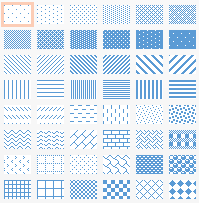
\includegraphics[scale=0.3]{figure.png}
		\caption{tiles}
		\label{fig:fig1}
	\end{figure}
	\begin{table}[H]
  		\caption{Dummy table}
	\end{table}
	
	\newpage
	%http://www.latex-tutorial.com/tutorials/beginners/latex-bibtex/
	%bibliography{
	
	\newpage
	\begin{appendix}
		\listoffigures
		\listoftables
	\end{appendix}
\end{document}

